\section{Galaxy Simulations}
The parameters of the spiral galaxy model, the configuration of the methods used in the simulation, and the results are provided below in raw form.
\subsection{\texorpdfstring{\PThreeM{}}{P3M} method}
\begin{table}[H]
    \centering
    \caption{\PThreeM{} method configuration.}
    \label{tab:p3m-method-parameters}
    \begin{tabular}{lc}
        \toprule
        \textbf{Parameter}      & \textbf{Value}           \\
        \midrule
        Effective mesh size     & $64 \times 64 \times 32$ \\
        $H$ (cell size)         & $60/64=0.9375$ kpc       \\
        DT (time step)          & $1$ Myr                  \\
        Mass assignment scheme  & TSC                      \\
        Finite difference       & Two-point                \\
        Time integration method & Leapfrog                 \\
        Number of particles     & 50,000                   \\
        $a$ (particle diameter) & $3H$                     \\
        Particle shape          & $S_1$                    \\
        $r_e$ (cutoff radius)   & $0.7a$                   \\
        \bottomrule
    \end{tabular}
\end{table}

\begin{figure}[H]
    \centering
    \begin{subfigure}[b]{0.45\textwidth}
        \centering
        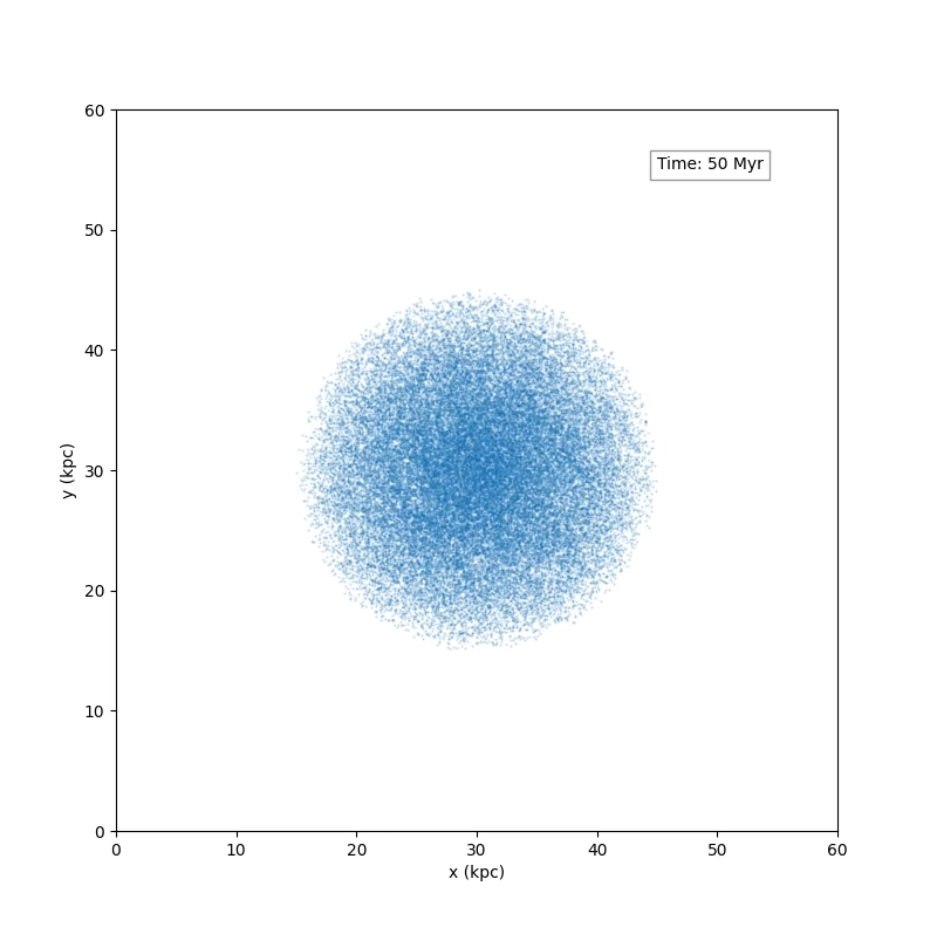
\includegraphics[width=\textwidth]{chapters/results/img/p3m-galaxy/50myr.png}
        \caption{$t=50\,\text{Myr}$}
        \label{fig:spiral-galaxy-evolution-p3m-sub1}
    \end{subfigure}
    \hfill
    \begin{subfigure}[b]{0.45\textwidth}
        \centering
        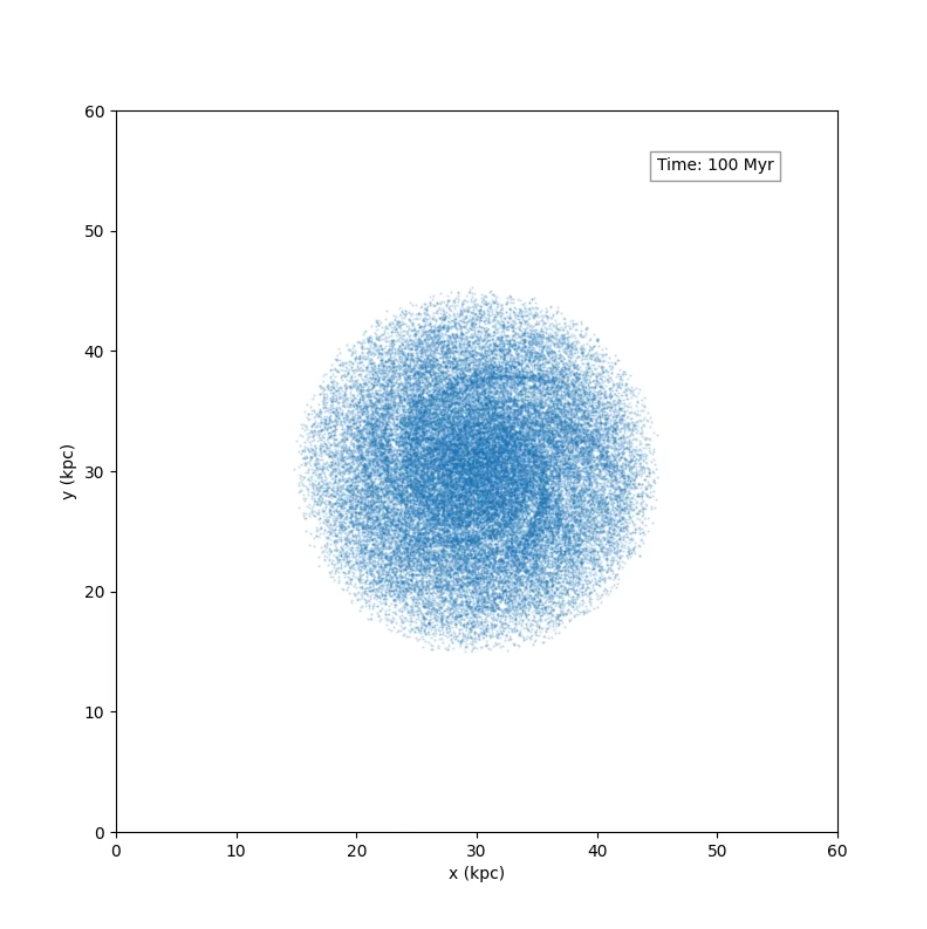
\includegraphics[width=\textwidth]{chapters/results/img/p3m-galaxy/100myr.png}
        \caption{$t=100\,\text{Myr}$}
        \label{fig:spiral-galaxy-evolution-p3m-sub2}
    \end{subfigure}

    \vspace{0.2cm}

    \begin{subfigure}[b]{0.45\textwidth}
        \centering
        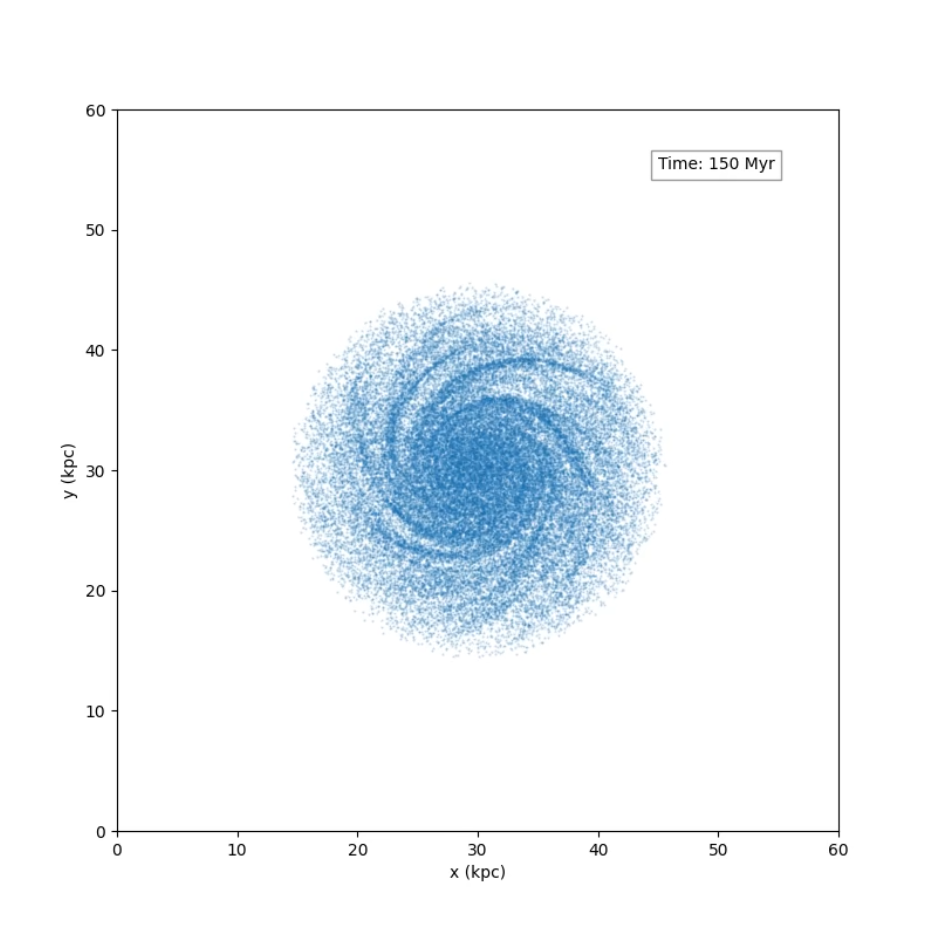
\includegraphics[width=\textwidth]{chapters/results/img/p3m-galaxy/150myr.png}
        \caption{$t=150\,\text{Myr}$}
        \label{fig:spiral-galaxy-evolution-p3m-sub3}
    \end{subfigure}
    \hfill
    \begin{subfigure}[b]{0.45\textwidth}
        \centering
        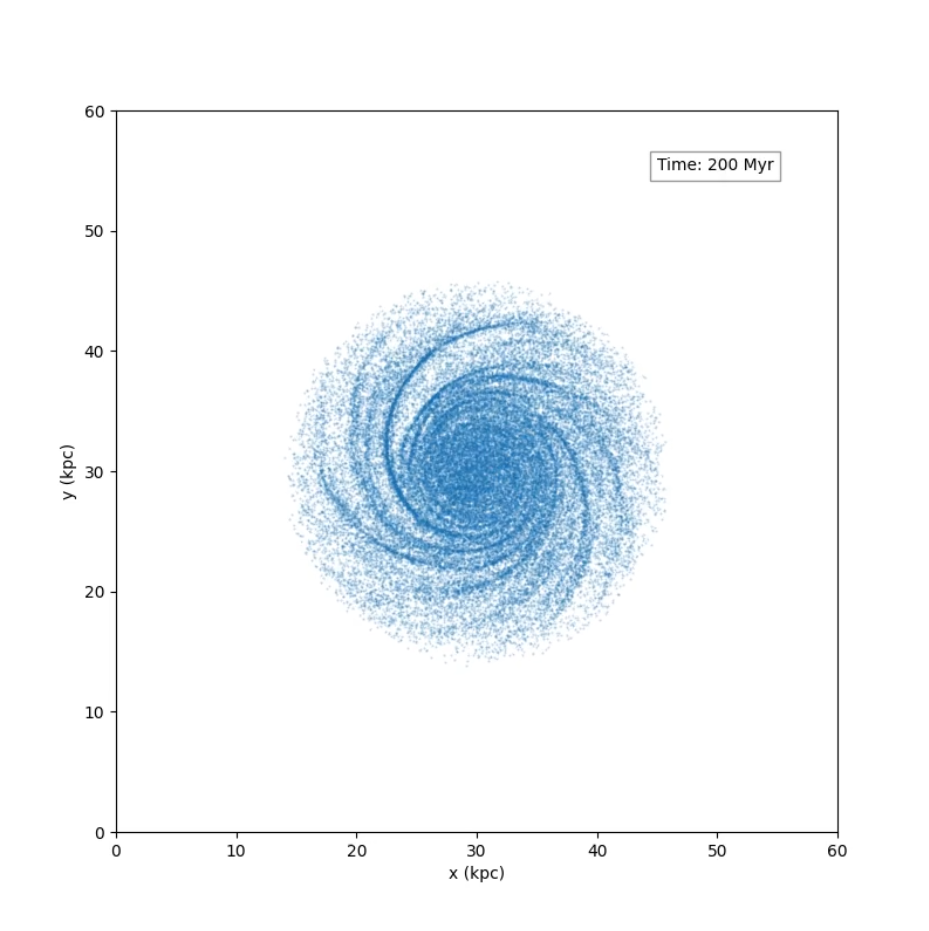
\includegraphics[width=\textwidth]{chapters/results/img/p3m-galaxy/200myr.png}
        \caption{$t=200\,\text{Myr}$}
        \label{fig:spiral-galaxy-evolution-p3m-sub4}
    \end{subfigure}

    \caption{Evolution of a spiral galaxy as predicted by the \PThreeM{} method.}
    \label{fig:spiral-galaxy-evolution-p3m}
\end{figure}

\begin{figure}[H]
    \centering
    \begin{subfigure}[b]{0.5\textwidth}
        \centering
        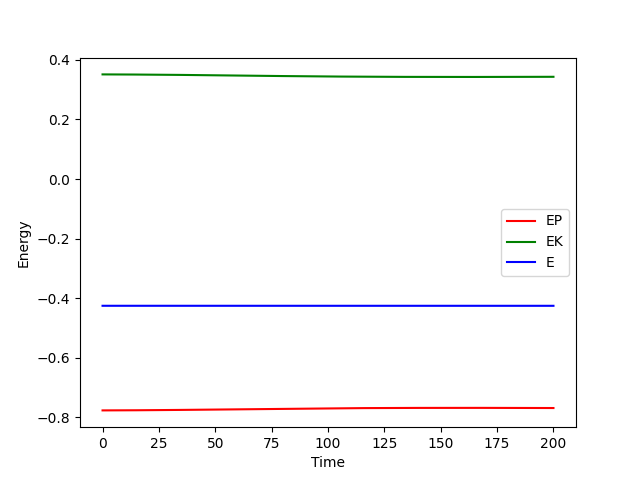
\includegraphics[width=\textwidth]{chapters/results/img/p3m-galaxy/energy.png}
        \caption{Energy}
        \label{fig:physical-quantities-p3m-sub1}
    \end{subfigure}

    \vspace{0.2cm}

    \begin{subfigure}[b]{0.5\textwidth}
        \centering
        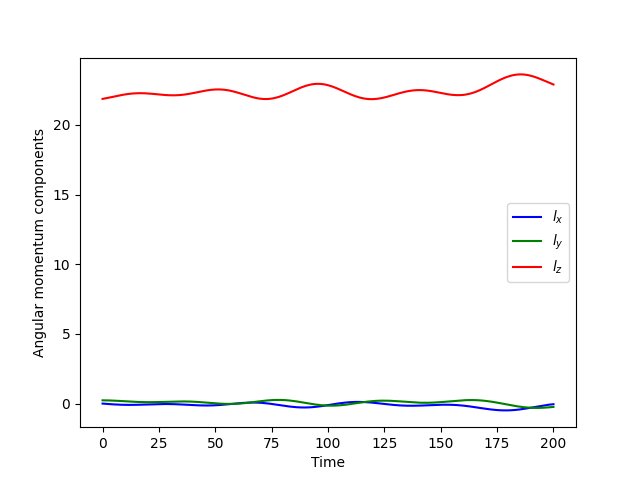
\includegraphics[width=\textwidth]{chapters/results/img/p3m-galaxy/angular-momentum.png}
        \caption{Angular momentum}
        \label{fig:physical-quantities-p3m-sub2}
    \end{subfigure}

    \vspace{0.2cm}

    \begin{subfigure}[b]{0.5\textwidth}
        \centering
        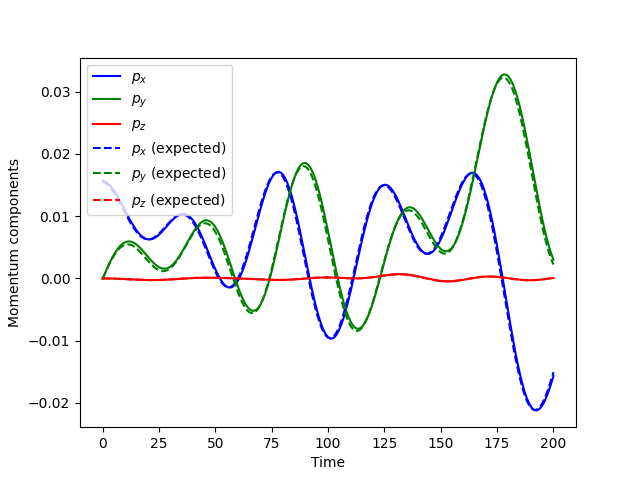
\includegraphics[width=\textwidth]{chapters/results/img/p3m-galaxy/momentum.png}
        \caption{Momentum; broken lines represent the expected momentum following \autoref{eq:expected-momentum-change}}
        \label{fig:physical-quantities-p3m-sub3}
    \end{subfigure}

    \caption{Fundamental physical quantities describing the system over time in the \PThreeM{} simulation.
        Time is in Myr and the quantities are expressed in units consistent with \autoref{tab:galaxy-parameters}}
    \label{fig:physical-quantities-p3m}
\end{figure}

\subsection{Barnes-Hut algorithm}
\begin{table}[H]
    \centering
    \caption{Barnes-Hut method configuration.}
    \label{tab:bh-method-parameters}
    \begin{tabular}{lc}
        \toprule
        \textbf{Parameter}            & \textbf{Value} \\
        \midrule
        $\theta$ (opening angle)      & 1              \\
        $\epsilon$ (softening length) & 1 pc           \\
        DT (time step)                & $1$ Myr        \\
        Highest multipole term        & monopole       \\
        \bottomrule
    \end{tabular}
\end{table}

\begin{figure}[H]
    \centering
    \begin{subfigure}[b]{0.45\textwidth}
        \centering
        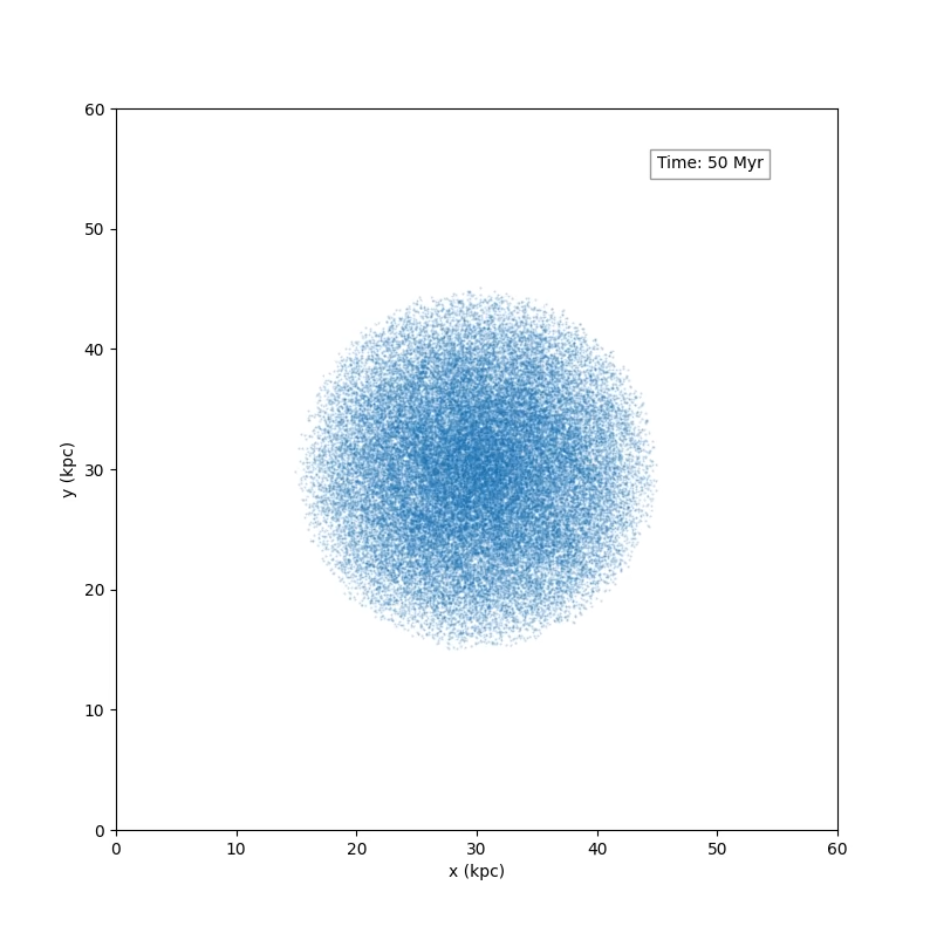
\includegraphics[width=\textwidth]{chapters/results/img/bh-galaxy/50myr.png}
        \caption{$t=50\,\text{Myr}$}
        \label{fig:spiral-galaxy-evolution-bh-sub1}
    \end{subfigure}
    \hfill
    \begin{subfigure}[b]{0.45\textwidth}
        \centering
        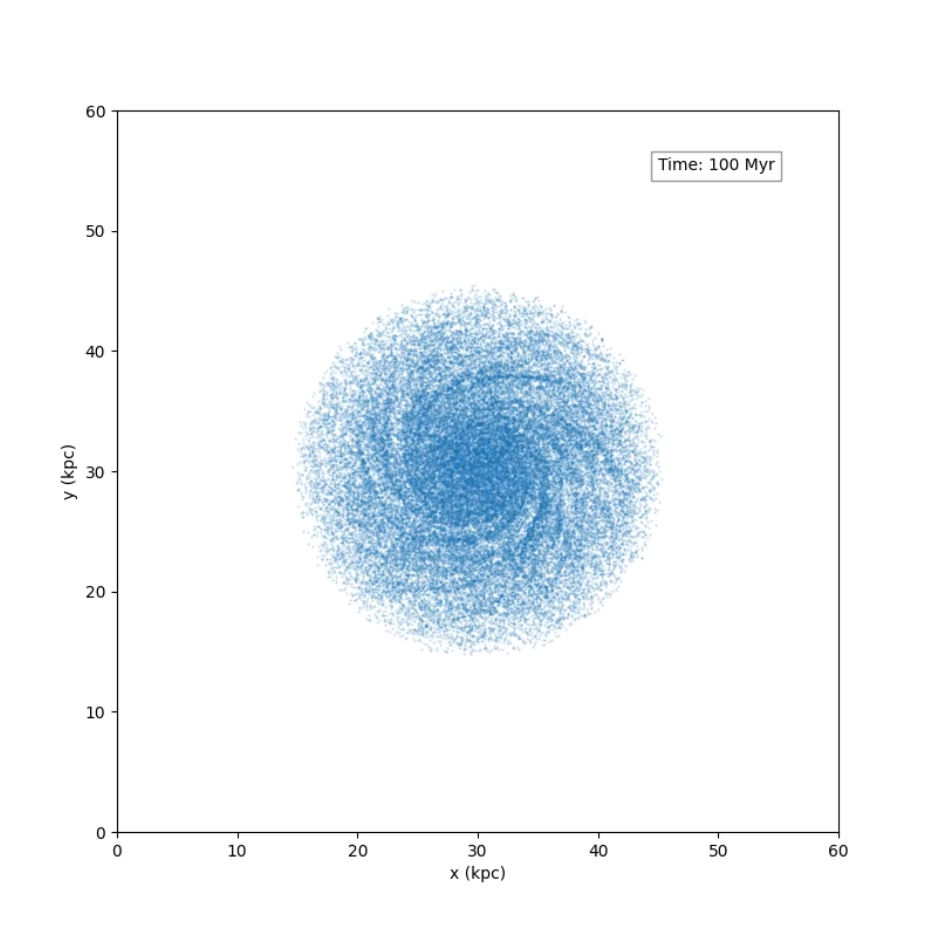
\includegraphics[width=\textwidth]{chapters/results/img/bh-galaxy/100myr.png}
        \caption{$t=100\,\text{Myr}$}
        \label{fig:spiral-galaxy-evolution-bh-sub2}
    \end{subfigure}

    \vspace{0.2cm}

    \begin{subfigure}[b]{0.45\textwidth}
        \centering
        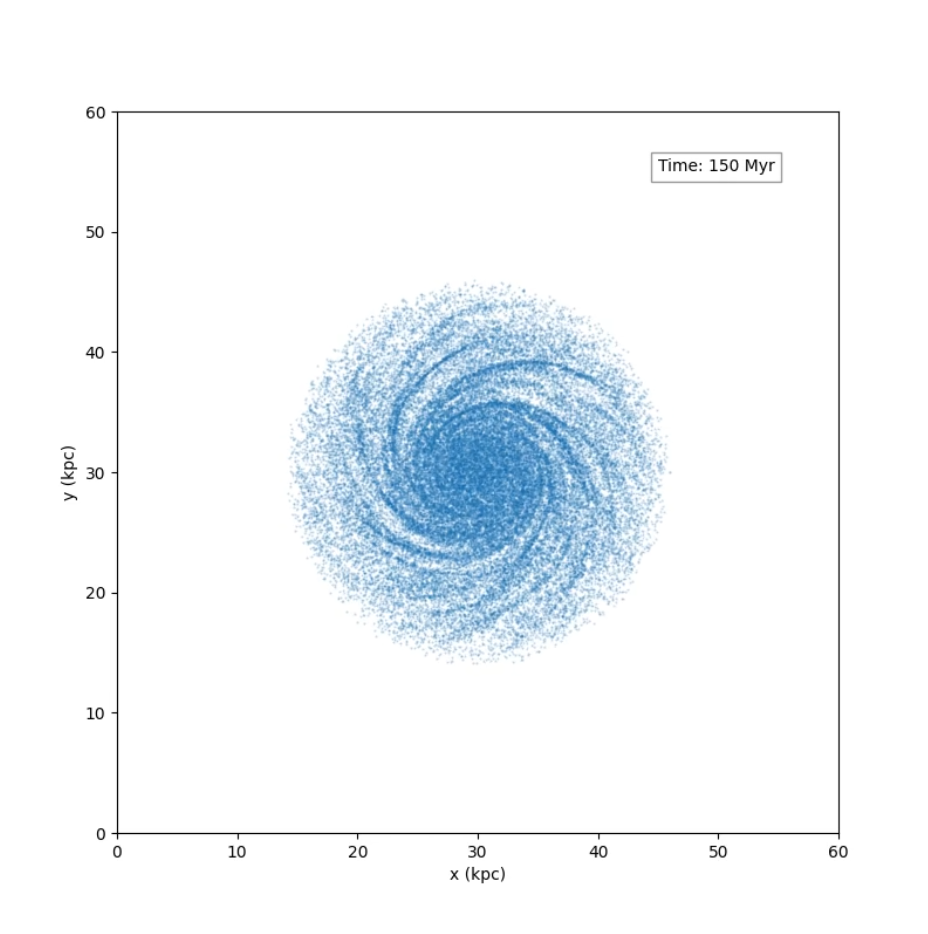
\includegraphics[width=\textwidth]{chapters/results/img/bh-galaxy/150myr.png}
        \caption{$t=150\,\text{Myr}$}
        \label{fig:spiral-galaxy-evolution-bh-sub3}
    \end{subfigure}
    \hfill
    \begin{subfigure}[b]{0.45\textwidth}
        \centering
        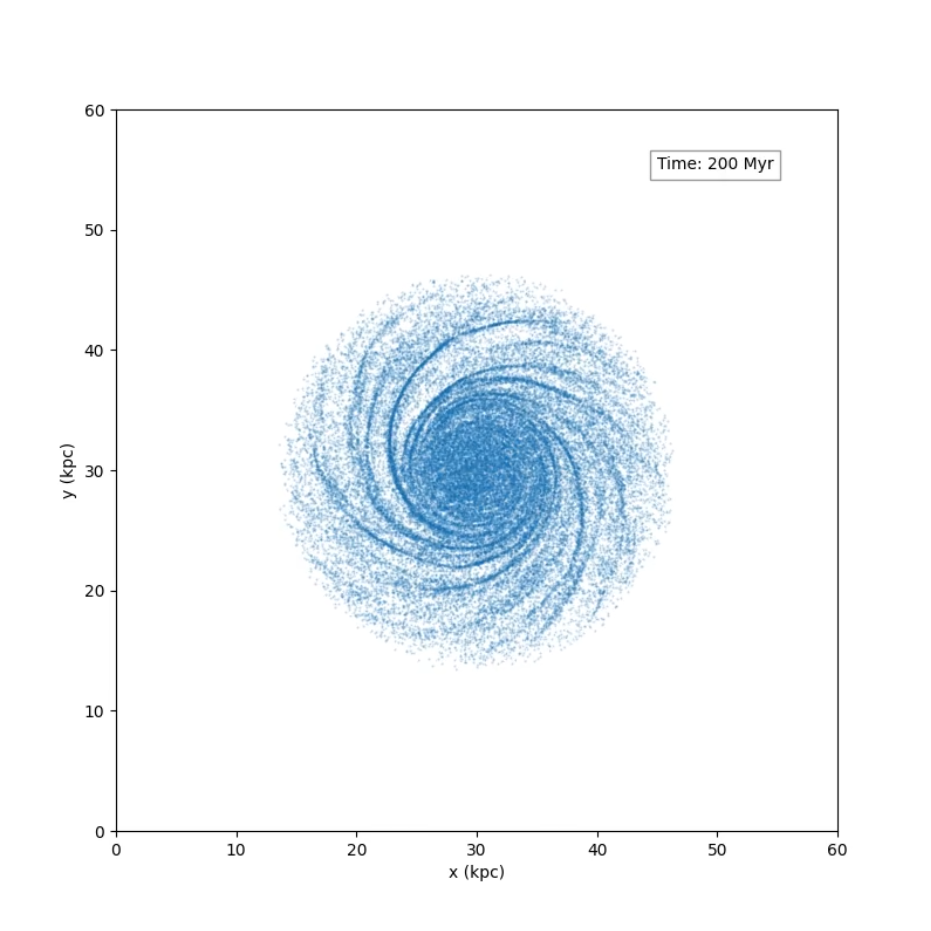
\includegraphics[width=\textwidth]{chapters/results/img/bh-galaxy/200myr.png}
        \caption{$t=200\,\text{Myr}$}
        \label{fig:spiral-galaxy-evolution-bh-sub4}
    \end{subfigure}

    \caption{Evolution of a spiral galaxy as predicted by the Barnes-Hut algorithm.}
    \label{fig:spiral-galaxy-evolution-bh}
\end{figure}

\begin{figure}[H]
    \centering
    \begin{subfigure}[b]{0.5\textwidth}
        \centering
        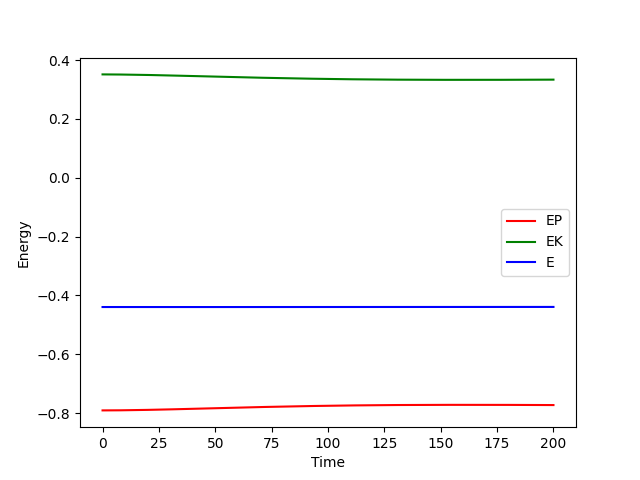
\includegraphics[width=\textwidth]{chapters/results/img/bh-galaxy/energy.png}
        \caption{Energy}
        \label{fig:physical-quantities-bh-sub1}
    \end{subfigure}

    \vspace{0.2cm}

    \begin{subfigure}[b]{0.5\textwidth}
        \centering
        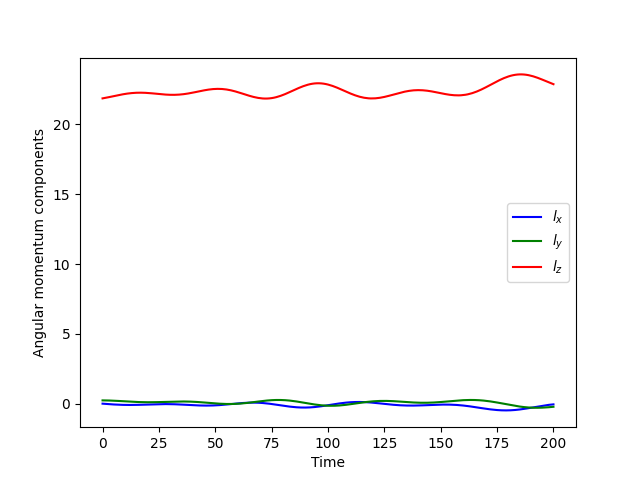
\includegraphics[width=\textwidth]{chapters/results/img/bh-galaxy/angular-momentum.png}
        \caption{Angular momentum}
        \label{fig:physical-quantities-bh-sub2}
    \end{subfigure}

    \vspace{0.2cm}

    \begin{subfigure}[b]{0.5\textwidth}
        \centering
        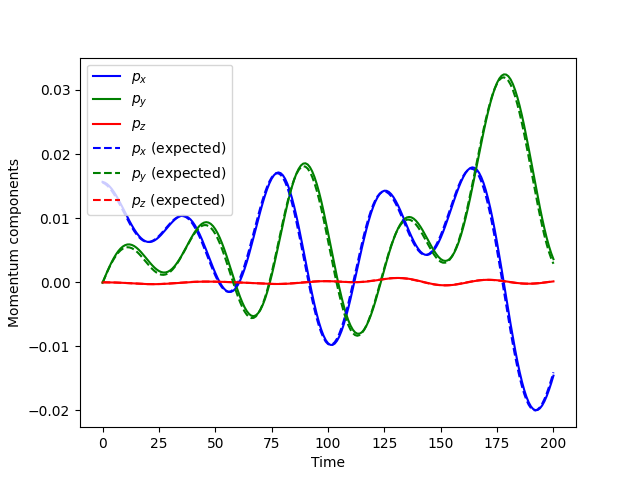
\includegraphics[width=\textwidth]{chapters/results/img/bh-galaxy/momentum.png}
        \caption{Momentum; broken lines represent the expected momentum following \autoref{eq:expected-momentum-change}}
        \label{fig:physical-quantities-bh-sub3}
    \end{subfigure}

    \caption{Fundamental physical quantities describing the system over time in the Barnes-Hut algorithm.
        Time is in Myr and the quantities are expressed in units consistent with \autoref{tab:galaxy-parameters}}
    \label{fig:physical-quantities-bh}
\end{figure}